\documentclass[a4paper]{article}
\usepackage{authblk}
\usepackage[pdftex]{graphicx}
\usepackage{sidecap}
\usepackage[T1]{fontenc}
\usepackage[utf8]{inputenc}
\usepackage[magyar]{babel}
\sloppy

\author{Andr\'as~Mameny\'ak}
\author{Roland~Bamli}
\affil{Mérnök informatikus szak (BSc), Debreceni Egyetem}

\title{Neurális hálózatok}

\begin{document}
\maketitle

\section{Bevezetés}
\subsection{A neurális hálózatok kialakulása}
A neurális hálózatok a mesterséges inteligencia egy típusa, amelyet az állatok központi idegrendszere, különösen az agy ihletett, amely képes a tanulásra, a mintafelismerésre is. Megalkotásához biológiai ismeretekre és az idegsejt működésének pontosabb megismerésére volt szükség. Ez csak a 20. században valósult meg. Az első neuron modelt 1947-ben alkotta meg McCullock és Pitts, az első mesterséges neuront pedig Rosenblatt 1958-ban. A neurális hálózatok egy ígéretes, új tudományterület, mely Webos 1974-es "back propagation" algoritmusa és annak 1986-os újra felfedezése után indult igazán fejlődésnek.

\subsection{Biológiai alapok}
Neuronnak nevezzük az idegsejt és az összes nyúlványainak együttesét.  
Állatfajonkénti és egy konkrét fajon belüli a különböző funkicók megvalósítása alapján megfigyelhető változatossága igen nagy. Felépítését tekintve minden neuronnál azonos, hogy négy fő része van,  a szóma, a dendritek, a myelin hüvely és az axon (1. ábra). A dentritek fogadják a bemeneti jeleket, melyetek az axon neurotransmitterekkel továbbit a következő idegsejt sejttestére és dendritjeire.

\begin{figure}[hb]
  \centering
  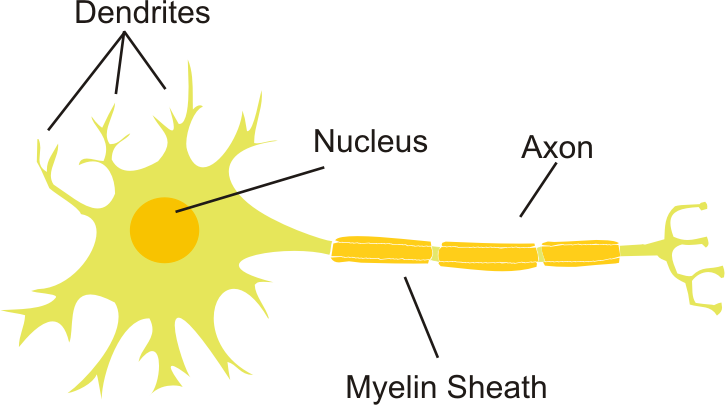
\includegraphics[width=0.7\textwidth]{neuron}
  \caption{\textit{Egy biológiai neuron felépítése.}}
\end{figure}

Tanulmányozásuk jelentős eredményekkel járhat, mivel jelenlegi ismereteink ezen a területen meglehetősen korlátozottak. Érdekesség képpen, az emberi agy több mint 100 milliárd neuronból áll. 

\subsection{A mesterséges neuron felépítése, működése}
Egy mesterséges neuron, mint a biológiai, több bemenettel és egy kimenettel rendelkezik (2. ábra). Egy általános neuron működése szerint  meghatározza a bemenetek súlyozott összegét és ezen végrehajt valamilyen nem lineáris leképezést. Ez utóbbit nevezik aktivációs, transzfer vagy aktiváló függvénynek. A végeredmény pedig a neuron kimeneti jele. Egy másik változat a lineráris összegzést megvalósító neuron, amikor nem történik lineáris leképezés.

\begin{figure}[hb]
  \centering
  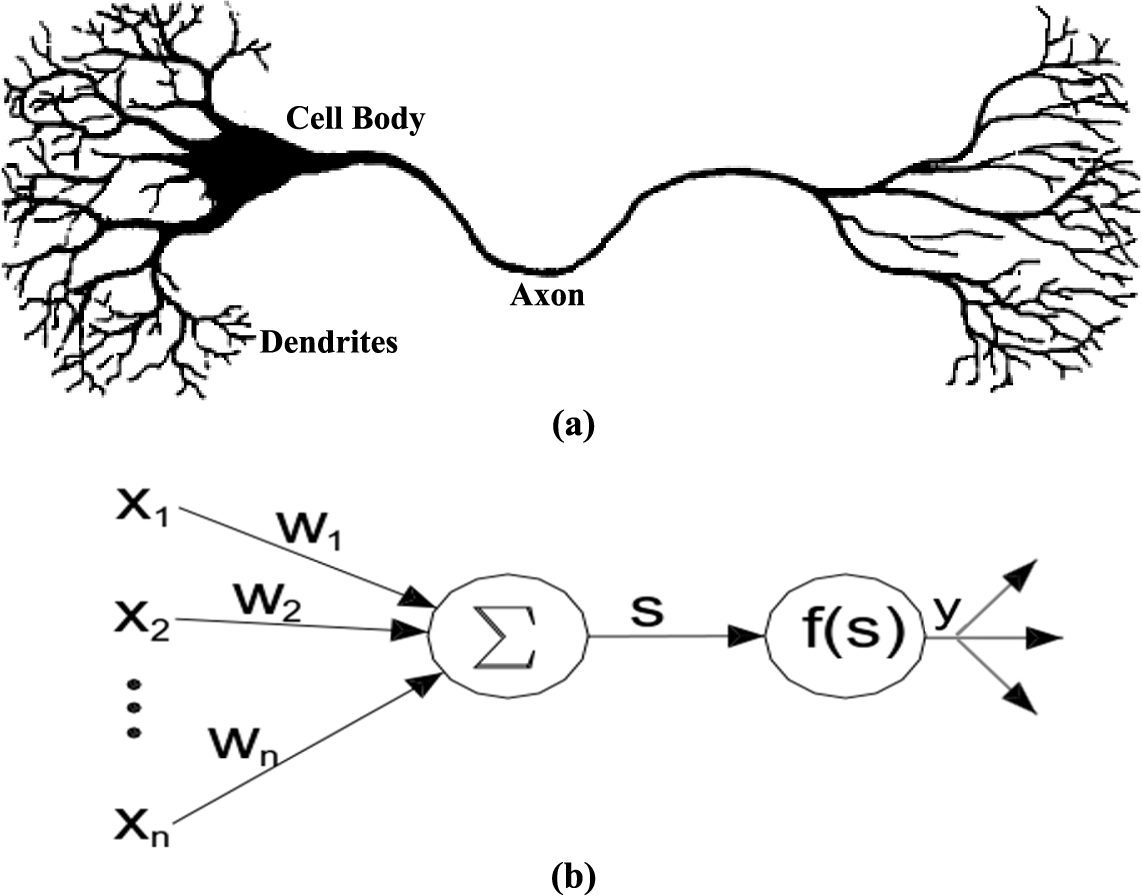
\includegraphics[width=0.6\textwidth]{artifical_neuron}
  \caption{\textit{A biológiai neuron (a) és a mesterséges neuron (b) összehasonlítása}}
\end{figure}

A 2. ábrán a neuron bemeneteit x${_i}$ jelöli, a kimeneti jel pedig y. Először a bemenetek súlyozott összegei kerülnek meghatározásra: $${s=\sum_{i=0}^{n} W_i \cdot x_i = W^T \cdot x}$$

Abban az esetben, ha a neuron lineáris összegzést valósít meg, ezzel már meg is kaptuk a kimeneti jelet:$${y = s = W^T \cdot x}$$

Nem lineáris esetben szükség van még a nem lineáris leképezésre. Ebben az esetben a neuron kimeneti jele a következő:$${y = f(s) = f(W^T \cdot x)}$$ ahol ${f(s)}$ az aktivizációs függvény. Erre a célra a négy leggyakrabban használt függvény a lépcső- vagy szignumfüggvény, a ``telítéses lineáris'' függvény, a tangens hiperbolikusz függvény és a szigmoid függvény.

Használnak egy másik elterjedt neuron típust is a RBF (Radial Bass Function) hálózatokban. Ennél a típusnál nincs lineáris összegzés,  az összes bemenet az aktivizációs függvénybe kerül, mely több bemenet esetén több változós függvény lesz.

\subsection{A neuron hálózatok felépítése}
A neuronokból álló hálózatokat nevezzük neurális hálózatoknak. Ezekben minden neuron ugyanolyan, vagy hasonló műveleteket végez, a többi neurontól függetlenül, lokálisan. Tehát ezek a hálózatok olyan információfeldolgozó eszközök, amelyek párhuzamos, elosztott működésre, tanulásra képesek. Általában irányított gráffal reprezentáljuk őket. A neuronok a gráf csomópontjai, míg a gráf élei a kimenetek és bemenetek közötti kapcsolatot reprezentálják. Megvalósíthatók szoftveresen, hardveresen, vagy a kettő kombinációjaként is. 

A neuronok három fajtáját különböztetjük meg:
\begin{enumerate}
    \item\textbf{bemeneti neuronok:} Egy bemenetű, egy kimenetű, buffer jellegű neuronok, jelfeldolgozó feladatuk nincs. Bemenetük a hálózat bemenete, kimenetük más neuronok meghajtására szolgál.
    \item\textbf{rejtett neuronok:} Ezek a neuronok végzik a jelfeldolgozást. Kimenetük és bemenetük is más neuronokhoz csatlakozik.
    \item\textbf{kimeneti neuronok:}A környezet felé továbbítják kimenetüket.
\end{enumerate}

A neuronokat álltalában típusa alapján rétegekbe szervezzük. Ennek megfelelően beszélhetünk bemeneti rétegről, retjett réteg(ek)ről és kimeneti rétegről.

A neuronhálózatokat az egyes neuronok közötti összeköttetési rendszer alapján két fő csoportba sorolhatjuk. Beszélhetünk előrecsatol hálózatokról és visszacsatolt hálózatokról. Akkor nevezünk egy neurálos hálózatot visszacsatoltnak, ha a topológiáját reprezentáló irányított gráf tartalmaz hurkot. Ez esetben beszélhetünk  globális és lokális visszacsatolásról.

\begin{figure}[hb]
  \centering
  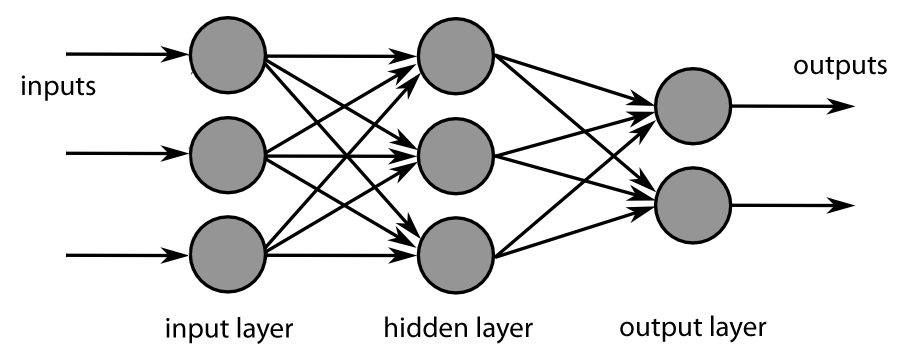
\includegraphics[width=1\textwidth]{neuron_layers}
  \caption{\textit{Előrecsatolt neuron hálózatok felépítése.}}
\end{figure}

\subsection{Back-propagation algoritmus}
A back-propagation, teljes nevén ``backward propagation of errors'', magyarul hiba-visszaterjesztési eljárás, egy tanulási algoritmust, melyet gyakran használnak a neurális hálózatokban. Ez egy felügyelt tanulási módszer, melynek szüksége van egy nagy adatbázisra a bemenetekkel és a kívánt kimenetekkel. Alkalmazása az előrecsatolt hálózatoknál a leghasznosabb. Használatához meg kell követelnünk, hogy a neuron hálózat réteges felépítésű, a neuron átviteli függvénye pedig deriválható legyen. Az algoritmusban a tanulás lényegében a hátrafelé terjedés folyamata, mely során minimalizálni kell az elvárt és a tényleges output vektor közötti négyzetes eltérést, Euklideszi távolságot.

Működése alapján két fázisra lehet osztani, terjedésre (propagation) és a súlyok frissítésére. A terjedés során a jel mind előre, mind hátra a szinapszisok és a neuronok szintjén lokális információk alapján terjed. A súlyok frissítése a neuron kimenetére visszaérkezett jel alapján történik.

\begin{figure}[hb]
  \centering
  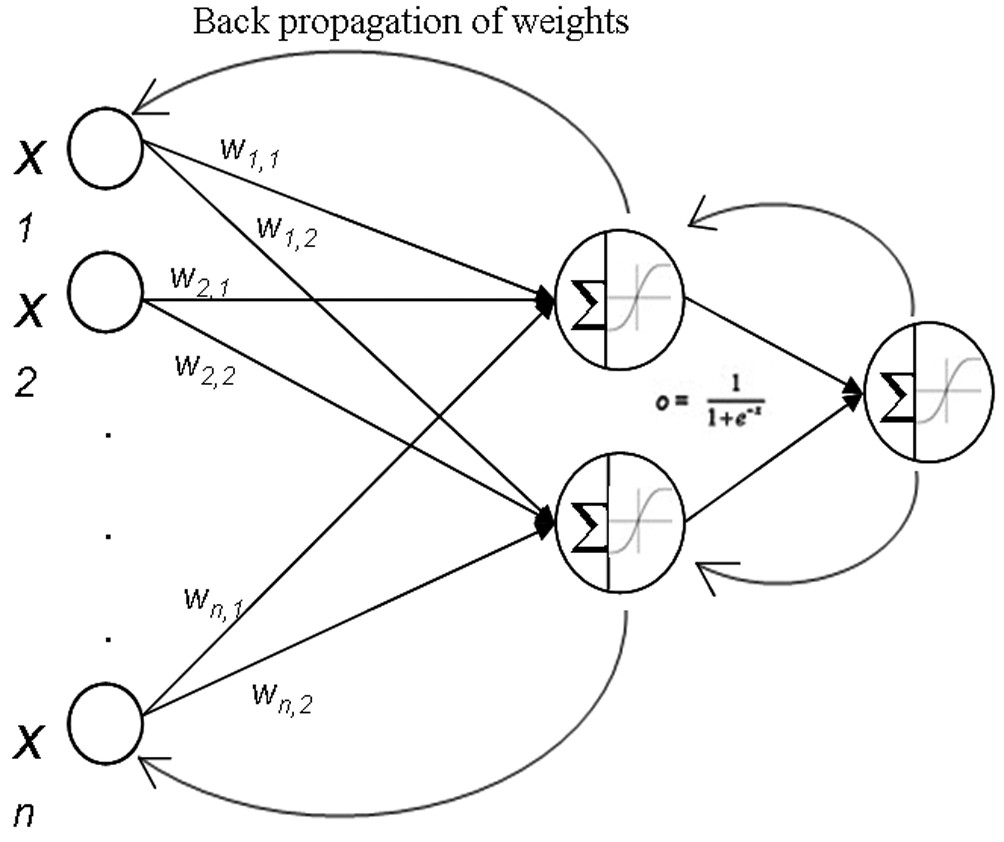
\includegraphics[width=0.8\textwidth]{backpropagation}
  \caption{\textit{A back-propagation algoritmus működése.}}
\end{figure}

\section{Conclusion}

\end{document}
